%\subsection{Билет 41 Объясненные	каноническими	переменными	доли	дисперсии.	Избыточность.}
%Пусть $\overline{\xi} \in \R^p, \ \overline{\eta} \in \R^q$ --- исходные признаки.
%$A_i^T \overline{\xi}, \ B_i^T \overline{\eta}$ --- $i$-ые канонические направления.
%Утверждается, что, если $\mathbb{E}\xi_i = 0, \mathbb{D}\xi_i = 1, \ \mathbb{E}\eta_i = 0, \mathbb{D}\eta_i = 1 \ \forall i$, то
%\begin{equation*}
%\sum\limits_{k = 1}^{s} \rho^2(\eta_i, B_k^T \overline{\eta}) \le 1 = \mathbb{D}\eta_i, \ \sum\limits_{k = 1}^{s} \rho^2(\xi_i, A_k^T \overline{\xi}) \le 1 = \mathbb{D} \xi_i , \ s = \min(p, q).
%\end{equation*}
%При этом, если $s = q$, то в первом случае достигается равенство, а если $s = p$, то во втором.
%Поэтому $\sum\limits_{k = 1}^{s} \rho^2(\eta_i, B_k^T \overline{\eta})$ и $\sum\limits_{k = 1}^{s} \rho^2(\xi_i, A_k^T \overline{\xi})$ называется объясненной долей дисперсии.
%
%\textbf{Избыточность:}
%Избыточностью $i$-ого левого признака $\xi_i$ называется
%\begin{equation*}
%\sum\limits_{k = 1}^{s} \rho^2(\xi_i, B_k^T \overline{\eta}).
%\end{equation*}
%Аналогично для правых. На консультации мы не разобрались, как ее интерпретировать, поэтому достаточно только определения.

%\subsection{Билет 42.Что общего	между	дискриминантным	анализом в многомерной	множественной	регрессией?}
%Окей, давайте по порядку.
%Задача MANOVA (буду сразу писать в нормальной модели с равными ковариационными матрицами, а не начинать с общей задачи на равенство распределений):
%
%Пусть $\eta_i \sim \mathcal{N}(\mu_i, \Sigma)$, $i = 1, \ldots k$.
%
%Необходимо проверить гипотезу
%\begin{equation*}
%H_0: \mu_1 = \ldots = \mu_k.
%\end{equation*}
%Введем одномерный качественный признак $\xi$, принимающий значения $A_1, \ldots A_k$. Тогда можно рассмотреть пару $(\eta, \xi)$, такую что $\mathcal{P}_{\eta \mid \xi = A_i} = \mathcal{P}_{\eta_i}$ и гипотеза принимает вид
%\begin{equation*}
%H_0: \mathbb{E}(\eta \mid \xi = A_1) = \ldots = \mathbb{E}(\eta \mid \xi = A_k).
%\end{equation*}
%Что эквивалентно независимости $\eta$ от $\xi$
%Знаем, что
%\begin{equation*}
%\mathbb{E}(\eta - \mathbb{E}\eta)(\eta - \mathbb{E}\eta)^T = \mathbb{E}(\mathbb{E}(\eta \mid \xi) - \mathbb{E}\eta)(\mathbb{E}(\eta \mid \xi) - \mathbb{E}\eta)^T + \mathbb{E}(\eta - \mathbb{E}(\eta \mid \xi))(\eta - \mathbb{E}(\eta \mid \xi))^T
%\end{equation*}
%То есть, на самом деле мы можем проверять гипотезу о том, что
%\begin{equation*}
%H_0: \mathbb{E}(\mathbb{E}(\eta \mid \xi) - \mathbb{E}\eta)(\mathbb{E}(\eta \mid \xi) - \mathbb{E}\eta)^T = 0
%\end{equation*}
%Теперь перейдем на выборочный язык и напишем основное дисперсионное тождество ($n_i$ -- длина выборки для $i$-ой группы.
%\begin{equation*}
%\sum\limits_{i = 1}^{k}\sum\limits_{j = 1}^{n_i}(y_{ij} - \overline{y})^2 = \sum\limits_{i = 1}^{k}n_i(y_{ij} - \overline{y}_{i.})^2  + \sum\limits_{i = 1}^{k}\sum\limits_{j = 1}^{n_i}(\overline{y}_{i.} - \overline{y})^2 = \mathbf{H} + \mathbf{E}
%\end{equation*}
%Статистика критерия, проверяющая нашу гипотезу имеет вид
%\begin{equation}
%\Lambda = \frac{|\mathbf{E}|}{|\mathbf{E} + \mathbf{H}|} = \prod\limits_{i = 1}^s (\frac{1}{1 + \lambda_i}),
%\label{maov}
%\end{equation}
%где $\lambda_i$ -- собственные числа матрицы $\mathbf{E}^{-1} \mathbf{H}$, $s = \min(p, k-1).$
%
%Теперь введем переменные $\zeta_1, \ldots, \zeta_{k-1}$ как dummy variables для переменной $\xi$ и рассмотрим многомерную множественную линейную регрессию вектора $\overline{\zeta}$ на $\eta$.
%А именно рассмотрим
%\begin{equation*}
%\mathbf{Y} = \mathbf{X}\mathbf{B} + \Xi
%\end{equation*}
%Предположим, что $\mathbf{Y}$ и $\mathbf{X}$ --- центрированы.
%Решение данной задачи $\hat{\mathbf{B}} = (\mathbf{X}^T\mathbf{X})^{-1}\mathbf{X}^T \mathbf{Y}$.
%Значимость регрессии проверяется гипотезой
%\begin{equation*}
%H_0: \mathbf{B} = 0.
%\end{equation*}
%Положим $\mathbf{E} = (\hat{\mathbf{Y}} - \mathbf{Y})(\hat{\mathbf{Y}} - \mathbf{Y})^T$,
%$\mathbf{H} = \hat{\mathbf{Y}}\hat{\mathbf{Y}} ^T$ и статистика критерия имеет вид
%\begin{equation}
%\Lambda = \frac{|\mathbf{E}|}{|\mathbf{E} + \mathbf{H}|} = \prod\limits_{i = 1}^s \left(\frac{1}{1 + \lambda_i}\right) = \prod(1 - r^2_i),
%\label{regr}
%\end{equation}
%где $r_i$ --- это $i$-ая каноническая корреляция.
%Так вот, оказывается, что $\Lambda$ из \eqref{maov} совпадает с  $\Lambda$ из $\eqref{regr}$.
%Таким образом получается, что $i$-ая каноническая корреляция между наборами $\zeta_1, \ldots, \zeta_{k-1}$ и $\eta_1, \ldots, \eta_p$ выражается через собственные числа $\lambda_i$, полученные в результате дискриминантного анализа как
%\begin{equation*}
%r_i^2 = \frac{\lambda_i}{1 + \lambda_i}
%\end{equation*}
%\subsection{Билет 43.Две группы, использование	множественной линейной регрессии для классификации.}
%Все в тех же обозначениях положим $k = 2$. Таким образом у нас получается только одна dummy-переменная и мы можем рассмотреть регрессию $\eta_1, \ldots, \eta_p$ на $\zeta_1$.
%(Мы все перевернули, но это не смертельно ибо в канонических корреляциях все симметрично).
%В таком случае первая каноническая корреляция $r^2_1 = R(\zeta, \eta_1, \ldots, \eta_p)$ --- это выборочный коэффициент корреляции.
%
%\begin{thm}
%Канонические коэффициенты $A_1$ пропорциональны $B^{(c)}$, которые получены при решении регрессионной задачи и пропорциональны $\Sigma^{-1}(\mu_1 - \mu_2)$.
%\end{thm}
%Вообще это частично показывалось, но я так поняла, что это не нужно..
%\newpage
\subsection{Кластерный анализ}

Цель кластерного анализа --- разбить индивиды на кластеры, т.е., на группы, между которыми, в некотором смысле,
расстояние больше, чем между точками внутри. Задача не формализована и, можно сказать, плохо поставлены,
 поэтому решается плохо.

Вообще, кластерный анализ --- это `обучение без учителя'. Это означает, что вы не сможете формально проверить правильность результата.

Единственный вариант поставить задачу четко --- это предположить какую-то статистическую модель данных и в ней находить
параметры, например, по методу максимального правдоподобия  (model-based clustering).

Все остальные методы --- эвристические с плохо определенным (хорошо-плохо) результатом.

\subsection{Кластерный	анализ,	пример	model-based	подхода}

Предположим, что многомерная выборка --- неоднородная. Но в отличие от дискриминантного анализа у нас нет признака, объясняющего эту неоднородность, и задачей является ее выявить.
Тип классификации, когда есть модель, называется model-based clustering.
Например, пусть наша выборка из смеси $k$ нормальных распределений. Таким образом ее плотность имеет вид
\begin{equation}
p(x) = \pi_1 p(x, \mu_1, \Sigma_1) + \ldots + \pi_k p(x, \mu_k, \Sigma_k),
\end{equation}
где
\begin{equation}
p(x, \mu_i, \Sigma_i) = \frac{1}{(2\pi)^{p/2}\sqrt{|\Sigma_i|}}
\exp \left(-\frac{1}{2}(x - \mu_i)\Sigma_i^{-1}(x - \mu_i)^T \right)
\end{equation}
Эта задача решается методом максимального правдоподобия. Можно выписать функцию правдоподобия (выпишите),
но она имеет сложный вид и искать ее максимум по такому большому числу параметров очень непросто.
Для нахождения этого максимума используется так называемый ЕМ-алгоритма (Expectation - Maximization).
Мы не будем здесь его обсуждать.



\subsection{Кластерный	анализ: $k$-means,	$k$-means$++$}
Хотим искать кластеры $C_1, \ldots, C_k$ минимизируя следующий функционал
\begin{equation}
\sum\limits_{i = 1}^k \sum\limits_{j \in C_i} ||x_j - \mu_i||^2
\label{func_lin}
\end{equation}
по разбиению всего пространства индивидов на $C_j$ и по всем $\mu_i$.
Можно делать это по следующему алгоритму:
\begin{enumerate}
\item Выбираем случайно $\mu_1, \ldots, \mu_k$.
\item $C_j$ -- кластер, содержащий точки, которые лежат к $\mu_j$ ближе, чем к остальным $\mu_i$.
\item Для каждого $C_j$ пересчитываем центр $\mu_j$ как выборочное среднее элементов из этого кластера.
\item Делаем 2 и 3 пока алгоритм не сойдется.
\end{enumerate}



\medskip
Проблема метода в том, что у такого функционала много локальных минимумов, и алгоритм может сойтись в значение, далекое от истинного.
Метод $k$-means$++$ повторяет алгоритм, приведенный выше, но начальные значения выбираются не случайно, а следующим образом
\begin{enumerate}
\item Выбираем случайным образом первый центр $\mu_1$.
\item Считаем расстояние от всех точек до ближайшего центра $\{\rho_i\}$. После чего выбираем $x_i$ как новый центр с вероятностью, пропорциональной $\rho_i$.
\item Пока количество центров меньше, чем $k$, повторяем процедуру.
\end{enumerate}
Результат функционала в $k$-means для данной процедуры выбора начальных центров запишем как $J(\{C_j\}, \{\mu_j\})$.
Известно, что при некоторых условиях на форму кластеров
\begin{equation*}
\frac{\mathbb{E}(J(\{C_j\}, \{\mu_j\}))}{J_{min}} = O(\ln k ),
\end{equation*}
т.е. результат, в среднем, довольно близко к настоящему минимуму.
%\subsection{Запись задачи, решаемой k-means, как задачи low-rank approximation с	ограничениями. Использование АГК}
%Функционал вида \eqref{func_lin} можно переписать в виде
%\begin{equation}
%    ||\mathbf{X} - \mathbf{G}\mathbf{M}||^2_F,
%\end{equation}
%где $M = (\mathbf{m}_1, \ldots, \mathbf{m}_k)$, $\mathbf{G}$ --- матрица, у которой в каждой строке
%стоит ровно одна единица и остальные нули.
%При этом, ранг матрицы $\mathbf{G}\mathbf{M}$ не превосходит $k$, что приводит нас к задачи
%аппроксимации заданной матрицы матрицей меньшего ранга.  Заметим, что задача похоже на задачу
%сингулярного разложения с ограничениями %\footnote{Матрица $\mathbf{G}$ должна «вытаскивать» вектор среднего для соответсвующей строчки $\mathbf{X}$}

\begin{note}
Есть результаты, что если к данным применить анализ главных компонент, то пространство, натянутое на первые $k-1$ главных векторов, при некоторых условиях будет близко к пространству, проходящему, через центры кластеров. Поэтому часто с помощью АГК уменьшают число признаков и потом применяют процедуру кластерного анализа.
\end{note}

\subsection{<<Плохие>> кластерные структуры}
	\begin{enumerate}
		\item
		\begin{tabular}{c c}
			\parbox{0.15\textwidth}{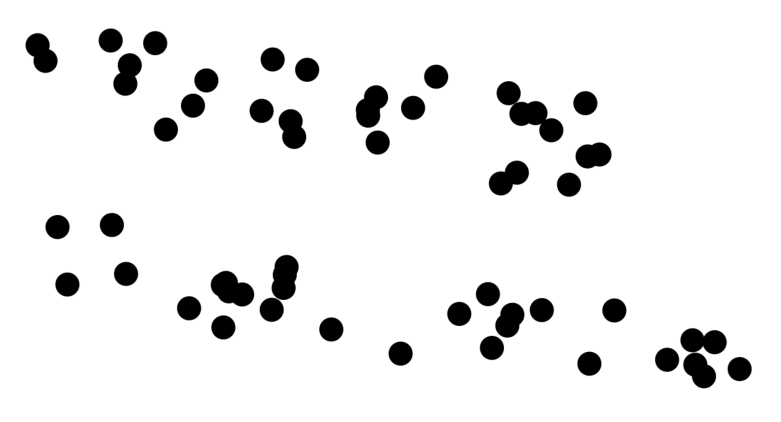
\includegraphics[width=0.15\textwidth]{img/lent.pdf}} & \parbox{0.7\textwidth}{ленточные кластеры. Внутрикластерные расстояния могут быть больше межкластерных;}
		\end{tabular}
		\vspace{0.5cm}
		\item
		\begin{tabular}{c c}
			\parbox{0.15\textwidth}{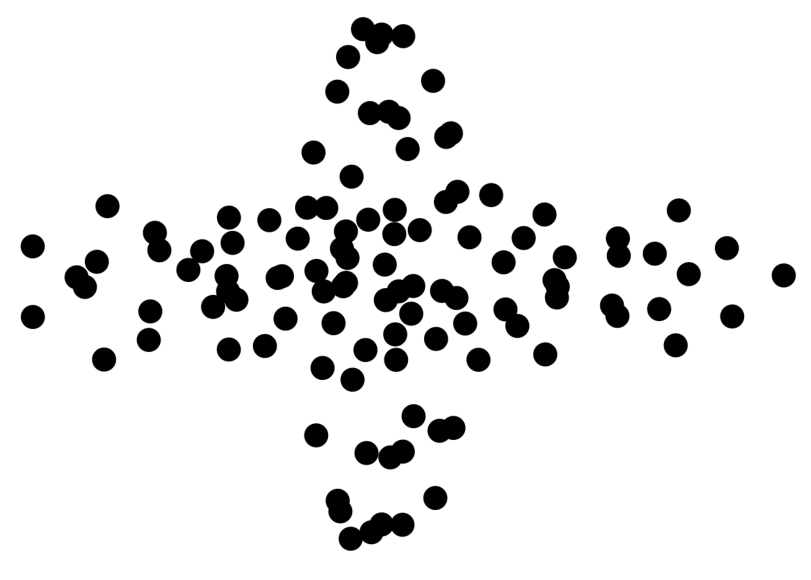
\includegraphics[width=0.15\textwidth]{img/perek.pdf}} & \parbox{0.7\textwidth}{перекрывающиеся кластеры;}
		\end{tabular}
		\vspace{0.5cm}
		\item
		\begin{tabular}{c c}
			\parbox{0.15\textwidth}{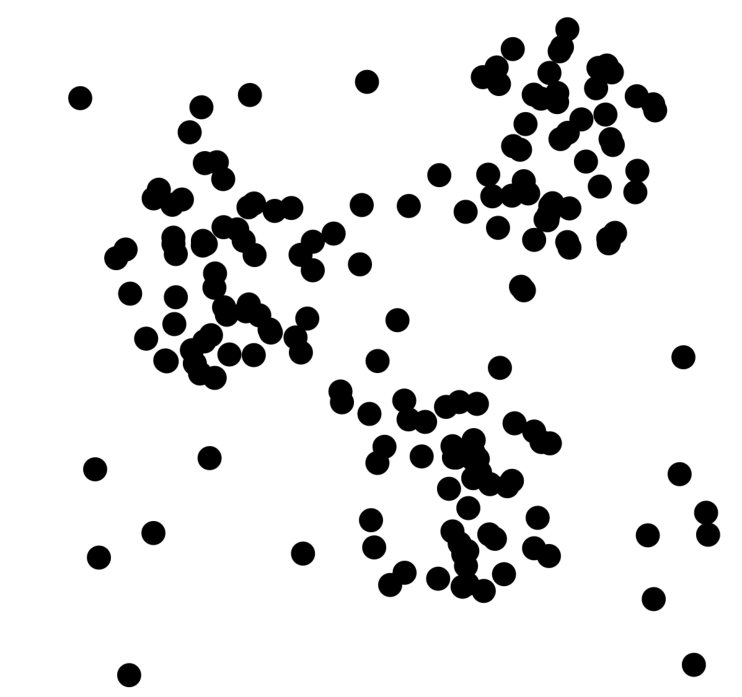
\includegraphics[width=0.15\textwidth]{img/fon.pdf}} & \parbox{0.7\textwidth}{кластеры, соединяющиеся перемычками и накладывающиеся на фон из редко расположенных объектов;}
		\end{tabular}
		\vspace{0.5cm}
		\item
		\begin{tabular}{c c}
			\parbox{0.15\textwidth}{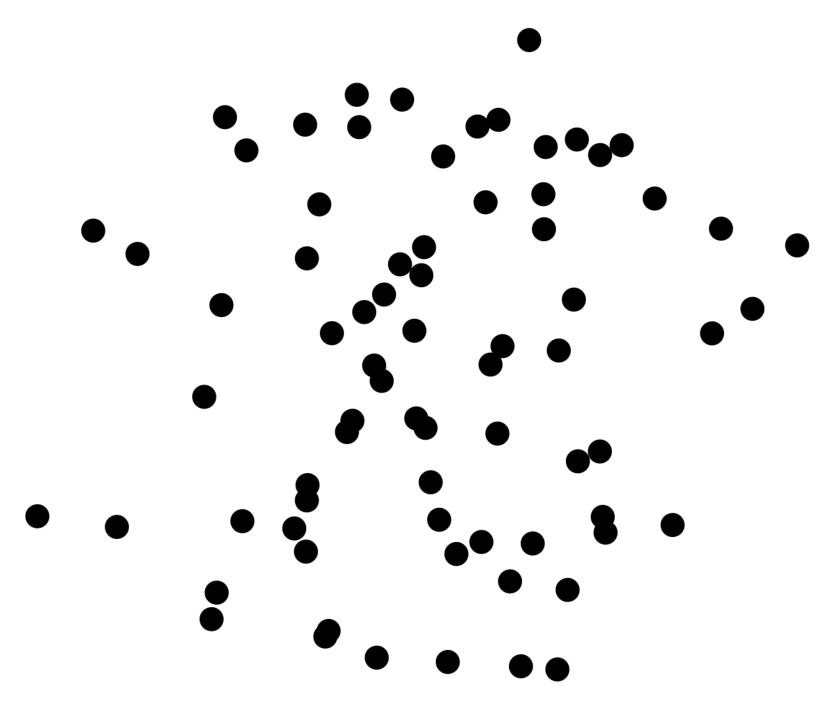
\includegraphics[width=0.15\textwidth]{img/ots.pdf}} & \parbox{0.7\textwidth}{кластеры могу отсутствовать.}
		\end{tabular}
	\end{enumerate}

Здесь мы обсуждали, что практически невозможно придумать определение кластера (не статистическое), при котором
все эти кластеры будут ему удовлетворять. Вариант смеси нормальных распределений, возможно, подойдет во всех случаях.

Еще обсуждали вопрос, что для данных, где реально обособленных кластеров может и не быть (например, последняя картинка),
часто кластеризацией называют сегментацию --- просто нарезку на части с описанием каждого сегмента на основе значений
признаков.

\subsection{Иерархический кластерный анализ}
\subsubsection{Расстояние между точками $\rho$}

Сначала нужно задать, как мы будем измерять расстояние между точками.

Самое стандартное --- евклидово расстояние: $\rho(x,y) = (\sum_i (x_i - y_i)^2 )^{1/2}$.

Расстояние городских кварталов (манхэттенское расстояние):  $\rho(x,y) = \sum_i |x_i - y_i|$.

Расстояние Чебышёва: $\rho(x,y) = \max_i |x_i - y_i|$.

Процент несогласия (эта мера используется в тех случаях, когда данные являются категориальными):
$\rho(x,y) = (\#\{i: x_i\neq y_i\}/ i$.

Особый случай, если кластеризуются признаки, а не индивиды (а какая разница --- такой кластерный анализ не статистическая процедура,
ему все равно), то логично в качестве расстояния рассматривать корреляции. Например, 1 минус модуль корреляции или
1 минус просто корреляция, что правильнее по смыслу для задачи.

\begin{note}
 Важно либо исходно стандартизовать признаки, либо измерять расстояние
специальным образом. Например, использовать расстояние Махаланобиса вместо обычного евклидового, если есть предположения о форме распределения точек внутри кластера.
\end{note}

\subsubsection{Примеры межкластерных расстояний}

Правила слияния кластеров (linkage rule) основывается на расстояниях между кластерами.

	% \setlength\arraycolsep{2pt}
	Расстояние ближнего соседа (single linkage, кластеры в виде цепочек):
	% ($\alpha_U=\alpha_V=\frac{1}{2}$, $\beta=0$, $\gamma=-\frac{1}{2}$)
	\[R^n(U,V)=\min_{u\in U,v\in V}\rho(u,v),\;U,V\subset X;\]

	расстояние дальнего соседа (complete linkage, кластеры ближе к шарикам):
	% ($\alpha_U=\alpha_V=\frac{1}{2}$, $\beta=0$, $\gamma=\frac{1}{2}$)
	\[R^l(U,V)=\max_{u\in U,v\in V}\rho(u,v);\]

	групповое среднее расстояние:
	%($\alpha_U=\frac{|U|}{|U \cup V|}$, $\alpha_V=\frac{|V|}{|U \cup V|}$, $\beta=\gamma=0$)
	\[R^g(U,V)=\frac{1}{|U||V|}\sum_{u\in U}\sum_{v\in V}\rho(u,v);\]

	расстояние между центрами:
	% ($\alpha_U=\frac{|U|}{|U \cup V|}$, $\alpha_V=\frac{|V|}{|U \cup V|}$, $\beta=-\alpha_U\alpha_V$, $\gamma=0$)
	\[R^c(U,V)=\rho^2\left(\sum_{u\in U}\frac{u}{|U|},\sum_{v\in V}\frac{v}{|V|}\right);\]

	расстояние Уорда:
	% ($\alpha_U=\frac{|U|}{|U \cup V|}$, $\alpha_V=\frac{|V|}{|U \cup V|}$, $\beta=-\alpha_U\alpha_V$, $\gamma=0$)
	\[R^w(U,V)=\frac{|U||V|}{|U|+|V|}R^c(U,V).\]


\subsubsection{Алгоритм агломеративной иерархической кластеризации}
	\begin{enumerate}
		\item Сначала все кластеры одноэлементные:
			$C_1=\left\{\{x_1\},\dots,\{x_l\}\right\}$; $R_1=0;$\\
			$\forall i\not=j$ вычислить $R\left(\{x_i\},\{x_j\}\right)$;
		\item\textcolor{blue}{для всех} $t=2,\dots,l$ (t -- номер итерации)
		\item\hspace{.5cm}найти в $C_{t-1}$ два ближайших кластера:\\
			\hspace{.5cm}$\displaystyle(U,V)=\argmin_{U \not= V}R(U,V);$\\
			\hspace{.5cm}$R_t=R(U,V);$
		\item\hspace{.5cm}слить их в один кластер:\\
			\hspace{.5cm}$W=U\cup V$;\\
			\hspace{.5cm}$C_t=C_{t-1}\cup W\setminus\{U,V\}$;
		\item\hspace{.5cm}\textcolor{blue}{для всех} $S \in C_t \setminus W$
		\item\hspace{1cm}вычислить $R(W,S)$;% по формуле Ланса--Уильямса;
	\end{enumerate}

\subsubsection{Визуализация кластерной структуры}
	\begin{dfn}
		Дендрограмма --- деревоподобный график, отражающий процесс последовательных слияний и структуру кластеров.
	\end{dfn}
	\begin{figure}[!h]
		%\subfigure{
			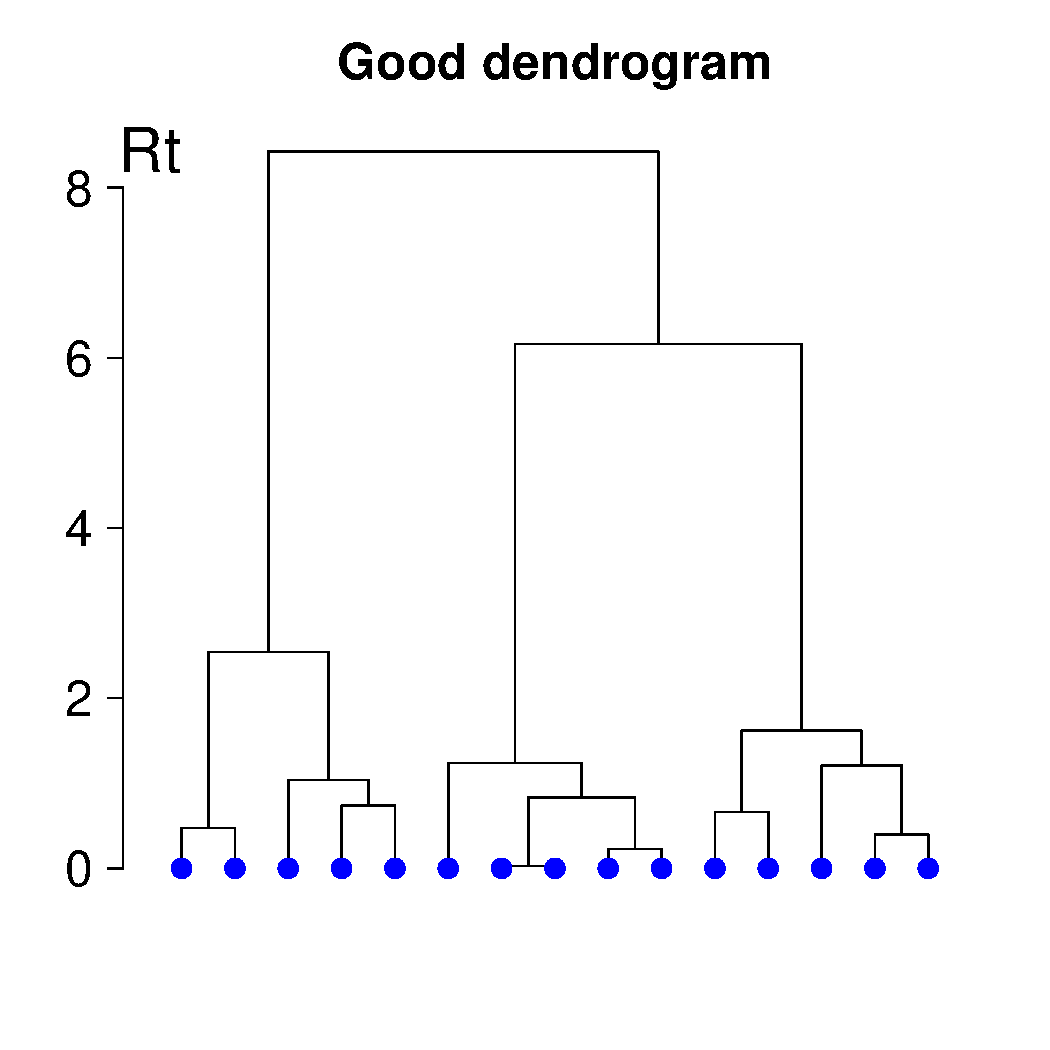
\includegraphics[width=0.4\textwidth]{img/ward.pdf}
			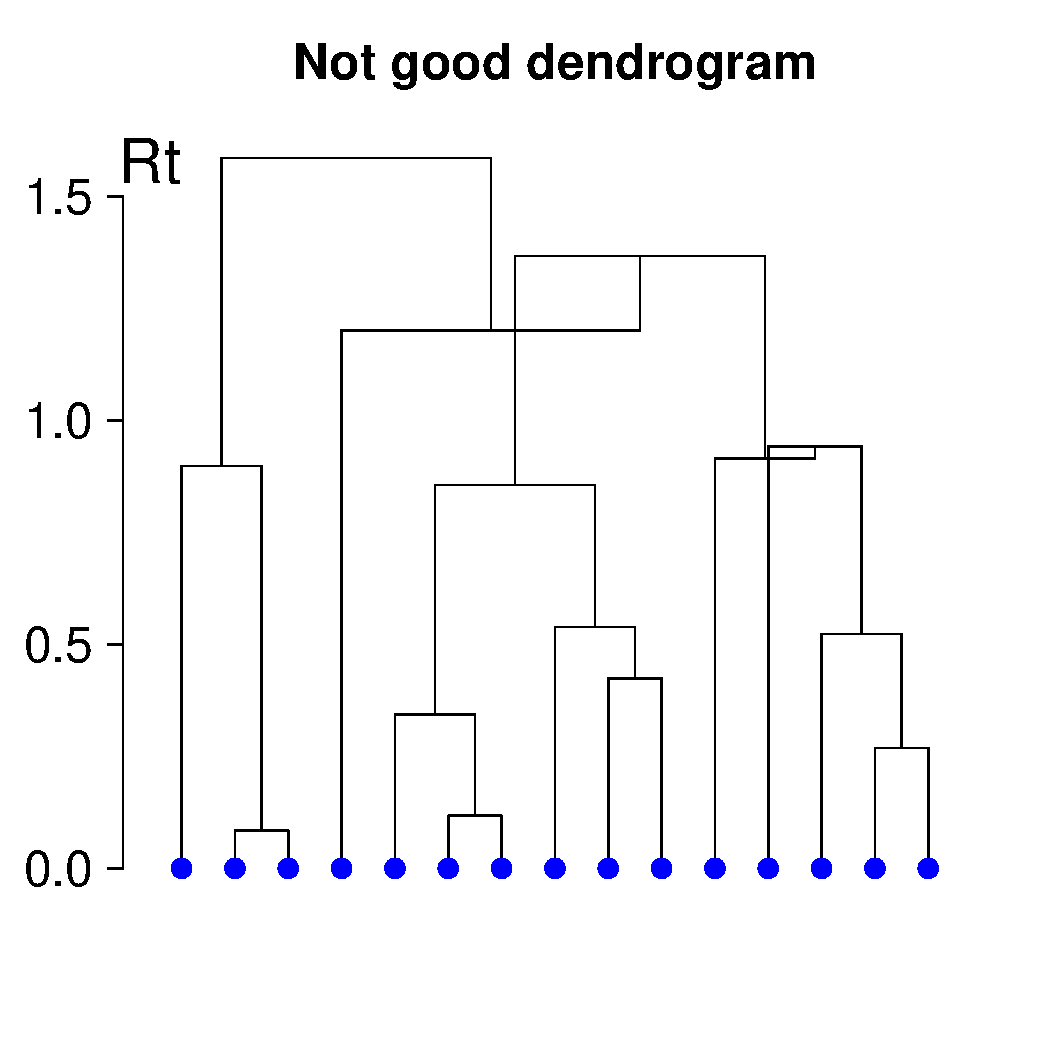
\includegraphics[width=0.4\textwidth]{img/centroid.pdf}
		%}
	\end{figure}

После построения дерева можно его разрезать на поддеревья по заданному расстоянию между кластерами
и получить сами кластеры. Разрез делается там, где долго не было объединения кластеров (длинная ветка у дерева).

Но долго-недолго  --- это субъективно и зависит от выбранного расстояния. Если расстояние в квадрате, то дальние
ветки искусственно удлиняются. 